\documentclass[12pt,a4paper,fontset=none]{ctexart}
\usepackage{ctex}
\usepackage{emptypage} 
\usepackage{fancyhdr}
\usepackage{amsmath,amsfonts,amssymb,mathtools}
\usepackage{graphicx}
\usepackage{mathptmx}
\usepackage{booktabs}
\usepackage[labelfont=bf]{caption}
\usepackage{indentfirst}
\usepackage{caption}
\usepackage{enumitem}
\usepackage[marginal]{footmisc}
\usepackage{subfigure}
\usepackage{fontspec}
\usepackage{geometry}
\usepackage{setspace}
\usepackage{listings}
\usepackage{xcolor}
\usepackage{tikz}
\usepackage{float}
\usepackage{pifont}
\usepackage{algorithm}
\usepackage{algorithmic}
\newgeometry{left=3cm,top=2.5cm,bottom=2.5cm,right=3cm}
\setmainfont{Times New Roman}
\setCJKmainfont[BoldFont=SimHei,ItalicFont=KaiTi]{SimSun}

\lstset{
	backgroundcolor=\color{green!10!blue!15},
	rulesepcolor= \color{red!40!blue!100},
	breaklines=true,
	breakatwhitespace=false,
	numbers=left, 
	numberstyle= \small,
	keywordstyle= \color{blue},
	commentstyle=\color{gray}, 
	frame=shadowbox
}

\renewcommand{\baselinestretch}{1.5}

\title{\textbf{概率论与数理统计第五次作业}}

\author{
\\
\Large{麻超 \quad 201300066}
\\[6pt]
{ \large \textit{南京大学人工智能学院}}\\[2pt]
}

\date{\today}
\newcommand{\supercite}[1]{\textsuperscript{\cite{#1}}}

\begin{document}
\maketitle
\setcounter{page}{1}

\section*{4.1.18}
X的分布函数为$F(x)=P(X\leqslant x)\cdot$

当x<0时,F(x)=0;

当$x> a$时,由题意可知F(x)=1.

当$0\leqslant x \leqslant a$时,由题意,$P(0\leqslant X \leqslant x)=kx.$

由于只在区间[0,a]上投掷,所以有$P(0\leqslant X\leqslant a)=ka=1$,故k=$\frac{1}{a} $.

所以得到:
\begin{align*}
    F(x)=
    \begin{cases}
        0,           & \text{} x<0            \\
        \frac{x}{a}, & \text{} 0\leqslant x<a \\
        1,           & \text{} x\geqslant a .
    \end{cases}
\end{align*}
\section*{4.1.19}
解:(1):P(至多三分钟)=$P(X\leqslant 3)=F_X(3)=1-e^{-1.2}$

(2):P(至少4分钟)=$1-P(X<4)=1-P(X\leqslant 4)=1-F_X(4)=e^{-1.6}$

(3):P(3-4分钟之间)=$P(3<X\leqslant 4)=F_X(4)-F_X(3)=e^{-1.2}-e^{-1.6}$

(4):P(至多4分钟或至少3分钟)=$1-P(3-4分钟之间)=1-e^{-1.2}+e^{-1.6}$.

(5):P(恰好2.5分钟)=0
\section*{4.1.20}
\subsubsection*{1}
$P(X<2)=P(X\leqslant 2)=F_X(2)=\ln 2$

$P(0<X\leqslant 3)=F_X(3)-F_X(0)=1$

$P(2<X<2.5)=P(2<X\leqslant 2.5)=F_X(2.5)-F_X(2)=\ln \frac{5}{2}-\ln 2=\ln \frac{5}{4}  $
\subsection*{2}
在$f_X(x)$的连续点处有$f_X(x)=\frac{d F_X(x)}{d x}$

故有:
\begin{align*}
    f_X(x)=
    \begin{cases}
        \frac{1}{x}, & \text{} 1<x\leqslant e                       \\
        0,           & \text{} x\leqslant 1\text{ } or\text{ } x< e
    \end{cases}
\end{align*}
\section*{4.1.21}
\subsection*{1}
由于概率密度函数f(x)在$(-\infty,1)\cup (2,\infty)$处都等于0,故有:

当x<1时,$F(x)=\int_{-\infty}^{x}f(x)dx =\int_{-\infty}^{x}  0dx =0$,

当x>2时,$F(x)=\int_{-\infty}^{x}f(x)dx =1-\int_{x}^{\infty}  0dx =1$,

当$x\in [1,2]$时
\begin{align*}
    F(x) & =\int_{-\infty}^{x}f(x)dx=\int_{-\infty}^{1}0dx+\int_{1}^{x} 2(1-\frac{1}{x^2})dx ) \\
         & =2(x+\frac{1}{x}\bigg|_{1}^x )=2(x+\frac{1}{x}-2 )
\end{align*}

所以分布函数F(x)是:
\begin{align*}
    F(x)=
    \begin{cases}
        0,                   & \text{} x<1             \\
        2(x+\frac{1}{x}-2 ), & \text{} 1\leqslant x <2 \\
        1,                   & \text{} x\geqslant 2
    \end{cases}
\end{align*}
\subsection*{2}
f(x)在x<0,$x\geqslant 2$处都等于0,故

当x<0时,F(x)=0,当x$\geqslant 2$时,F(x)=1.

当$0\leqslant x <1$时
\begin{align*}
    F(x)=\int_{-\infty}^{x} f(x)dx=\int_{0}^{x}x dx=\frac{x^2}{2}
\end{align*}

当$1\leqslant x<2$时
\begin{align*}
    F(x) & =\int_{-\infty}^{x}f(x)dx=\int_{0}^{1}x dx +\int_{1}^{x}(2-x)dx \\
         & =\frac{1}{2}+(2x-\frac{x^2}{2} )\bigg|_1^x=2x-\frac{x^2}{2}-1
\end{align*}

故所求分布函数为:
\begin{align*}
    F(x)=
    \begin{cases}
        0,                  & \text{} x<0             \\
        \frac{x^2}{2} ,     & \text{} 0\leqslant x <1 \\
        2x-\frac{x^2}{2}-1, & \text{}1\leqslant x<2   \\
        1,                  & \text{} x\geqslant 2
    \end{cases}
\end{align*}

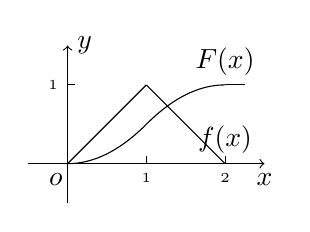
\begin{tikzpicture}
    \draw[->](-0.5,0)--(2.5,0) node[below] {$x$};
    %绘制(draw)x轴,线到箭头(->),从(-0.5,0)到(2.5,0),文字($x$)显示在下方(below)
    \draw[->](0,-0.5)--(0,1.5) node[right] {$y$};
    %绘制(draw)y轴,线到箭头(->),从(-0.5,0)到(1.5,0),文字($y$)显示在右侧(right)
    \draw plot[smooth, domain = 0:1] (\x,{\x}) node[above] {};
    \draw plot[smooth,domain=1:2](\x,{2-\x})node[above]{$f(x)$};
    \draw plot[smooth,domain=0:1](\x,{\x^2/2 })node[above]{};
    \draw plot[smooth,domain=1:2](\x,2*\x-\x^2/2-1 )node[above]{$F(x)$};
    \draw plot[smooth,domain=2:2.25](\x,1)node[above]{};
    %绘制(draw)x(\x)到y = f(x)({f(\x)()})的映射,平滑化(smooth),x取值范围为(0,1),文字($F(x)$)显示在上方(above)
    \foreach \x in {1,2} {\draw(\x,0)--(\x,0.1) node[below, font = \tiny] at(\x,0) {\x};}
    %x轴上的点:(1,0)、(2,0)(\foreach \x in {1,2}),在其位置(\x,0)绘制(draw)从(x,0)到(x,0.1),小字体(tiny),文字(\x)显示在下方(below)
    \foreach \y in {1} {\draw(0,\y)--(0.1,\y) node[left, font=\tiny] at(0,\y) {\y};}
    %y轴上的点:(0,1)(\foreach \y in {1}),在其位置(0,\y)绘制(draw)从(0,y)到(0.1,y),小字体(tiny),文字(\y)显示在下方(below)
    \draw(-0.15,0) node[below] {$o$};
    %在(-0.15,0)处绘制(draw)零点,字体($o$)显示在下方(below).
\end{tikzpicture}
\section*{4.1.23}
任取一只该种零件,其寿命大于1500h的概率为
\begin{align*}
    p=\int_{1500}^{\infty}\frac{1000}{x^2}dx=-\frac{1000}{x^2}\bigg|_{1500}^{\infty}=\frac{2}{3}
\end{align*}

记其中寿命大于1500小时的只数为X,则$X\sim b(5,2/3)$.

故所求概率为
\begin{align*}
    P(X\geqslant 2) & =1-P(X\geqslant 0)-P(X\geqslant 1)                         \\
                    & =1-(\frac{1}{3})^5-\binom{5}{1}\frac{2}{3}(\frac{1}{3} )^4 \\
                    & =\frac{232}{243}
\end{align*}
\section*{4.1.24}
顾客等待超过10min的概率为
\begin{align*}
    P=\int_{10}^{\infty}f_X(x)dx=\int_{10}^{\infty}\frac{1}{5}e^{-\frac{x}{5} } dx=e^{-2}
\end{align*}

故Y服从二项分布,即$Y\sim b(5,e^{-2})$.Y的分布律为
\begin{align*}
    P(Y=k)=\binom{5}{k} e^{-2k}(1-e^{-2})^{5-k},k=0,1,2,3,4,5 \\
    P(Y\geqslant 1)=1-P(Y=0)=1-(1-e^{-2})^5
\end{align*}
\section*{4.1.25}
若要让原式有实根,则需要满足$\Delta=16K^2-16K-32\geqslant 0$.

即需要满足$(K+1)(K-2)\geqslant 0$

解得$K\geqslant 2 $ or $ K\leqslant -1$

假设K在区间(0,5)上服从均匀分布,则有实根的概率$P=\frac{3}{5} $
\section*{4.1.18(P115)}
\begin{align*}
    E(x)=\int_{-\infty}^{\infty}xf(x)dx=\int_{0}^{\infty}\frac{x^2}{\sigma^2}e^{-\frac{x^2}{2\sigma^2} }
\end{align*}

令$t=x^2/(2\sigma^2)$,得到
\begin{align*}
    E(x) & =\sqrt2\sigma\int_{0}^{\infty}\sqrt te^{-t}dt
\end{align*}

令$\Gamma(\alpha)=\int_0^{\infty}x^{\alpha-1}e^{-x}dx$

则$\Gamma(\alpha+1)=\alpha\Gamma(\alpha)$

于是有
\begin{align*}
    E(X)   & =\sqrt 2\sigma\Gamma(\frac{1}{2} )=\sqrt 2\sigma\frac{1}{2} \Gamma(\frac{1}{2} )=\sqrt{\frac{\pi}{2} }\sigma \\
    E(x^2) & =\int_{-\infty}^{\infty}x^{2}f(x)dx
\end{align*}

同理可以得到
\begin{align*}
    E(X^2) & =2\sigma^2                                                             \\
    Var(X) & =E(X^2)-E(X)^2=2\sigma^2-\frac{\pi}{2}\sigma^2=\frac{4-\pi}{2}\sigma^2
\end{align*}
\section*{4.2}
设长方形的宽为b,长为a,则$a*b=10,a=\frac{10}{b} $

周长l=(a+b)*2=2(b+10/b).
所以\begin{align*}
    E(l)      & =2E(b)+2E(10/b)=2(E(b)+10E(b^{-1}))                                         \\
    E(b)      & =\frac{a+b}{2}=1                                                            \\
    E(b^{-1}) & =\int_{-\infty}^{\infty}t^{-1}f(t)dt=\frac{1}{2}\int_{0}^{2}t^{-1}dt=\infty
\end{align*}

所以$E(l)=\infty$

欲求方差,则因为$Var(x)=E(x^2)-E(x)^2$

\begin{align*}
    E(x^2)=\int_{-\infty}^{\infty}t^2f(t)dt=\frac{1}{2}\int_{0}^{2}t^2dt=\frac{3}{4}
\end{align*}

故其方差依然不存在.
\section*{4.3}
易知A一定大于0.
由于\begin{align*}
    \int_{-\infty}^{\infty}f(t)dt=\int_{0}^{\infty}Ae^{-t}dt=[-Ae^{-t}]_0^{\infty}=1
\end{align*}

故一定有A=1.

所以有当$x\geqslant 0$时,$f(x)=e^{-x}$.
\begin{align*}
    E(Y)=E(e^{-2x})=\int_{-\infty}^{\infty}e^{-x}\cdot e^{-2x}dx=-\frac{1}{3}e^{-3x}\bigg|_0^{\infty}=\frac{1}{3}
\end{align*}
\section*{4.4}
正态分布的随机变量X的概率密度满足
\begin{align*}
    f(x)=\frac{1}{\sqrt{2\pi}\sigma }e^{-\frac{(x-\mu )^2}{2\sigma^2} }
\end{align*}

由概率密度函数的规范性,考虑
\begin{align*}
    \int_{-\infty}^{\infty}\frac{1}{\sqrt{2\pi}\sigma }e^{-\frac{(x-\mu )^2}{2\sigma^2} }=1
\end{align*}
考虑到在固定的正态分布中,$\mu,\sigma$都是确定的值,故原式与下式相等
\begin{align*}
    \frac{1}{\sqrt{2\pi}\sigma }\int_{-\infty}^{\infty}e^{-\frac{(x-\mu )^2}{2\sigma^2} }
\end{align*}

令$(x-\mu)/\sigma=t$,得到:
\begin{align*}
     & \frac{1}{\sqrt{2\pi}\sigma }\int_{-\infty}^{\infty}e^{-\frac{(x-\mu )^2}{2\sigma^2} } \\=&\frac{1}{\sqrt{2\pi}}\int_{-\infty}^{\infty}e^{-\frac{t^2}{2} }dt\\=&\frac{1}{2\pi}\cdot I\\
     & I^2=\int_{-\infty}^{\infty}\int_{-\infty}^{\infty}e^{-(t^2+\mu^2)/2}dtdu
\end{align*}

利用极坐标转化为累次积分,得到
\begin{align*}
    I^2=\int_{0}^{2\pi}\int_{0}^{\infty}re^{-r^2/2}drd\theta=2\pi
\end{align*}

由于I>0,故$I=\sqrt{2\pi}$,即
\begin{align*}
    \int_{-\infty}^{\infty}e^{-t^2/2}dt=\sqrt{2\pi}
\end{align*}

所以有
\begin{align*}
    \frac{1}{\sqrt{2\pi}\sigma }\int_{-\infty}^{\infty}e^{-\frac{(x-\mu )^2}{2\sigma^2} }dx=\frac{1}{\sqrt{2\pi}}\int_{-\infty}^{\infty}e^{-t^2/2}dt=1
\end{align*}

于是有
\begin{align*}
    \frac{1}{\sqrt{2\pi}\sigma }=\int_{-\infty}^{\infty}e^{-\frac{(t-\mu )^2}{2\sigma^2} }dt
\end{align*}

\end{document}